\documentclass[9pt]{beamer}
\usetheme{boxes}
\usetheme{Boadilla}
\usecolortheme{beaver}
%\usecolortheme{sidebartab}
% \usefonttheme{structurebold}
\usefonttheme{serif}

%gets rid of bottom navigation bars
\setbeamertemplate{footline}[page number]{}

%gets rid of navigation symbols
\setbeamertemplate{navigation symbols}{}


% \usepackage{helvet}
\usepackage{amsmath, amssymb}
\usepackage{color}
%\usepackage{asymptote}
\usepackage{mathrsfs}
\usepackage{dsfont}
\usepackage{url}
\usepackage{cancel}
\usepackage{tikz}
\usetikzlibrary{fit,positioning}
\usetikzlibrary{shapes,matrix,decorations.markings,arrows}
\usetikzlibrary{graphs}
\usepackage{bbm}
\def\ind{\mathbbm{1}} %Indicator function


%
\definecolor{darkblue}{rgb}{0.0, 0.0, 0.55}
\setbeamercolor{title}{fg=darkblue}
\setbeamercolor{frametitle}{fg=darkblue}
\newcommand{\myitem}{\item[$\bullet$]}
\definecolor{darkgreen}{rgb}{0, 0.55, 0}


\newcommand{\LABEQ}[1]{\label{eq:#1}}%\mathtt{[eq:#1]}\qquad
\newcommand{\LABALG}[1]{\label{alg:#1}}%\mathtt{[lab:#1]}\qquad
\newcommand{\LABTAB}[1]{\label{tab:#1}}%{\tt [tab:$\text{$#1$}$]}}
\newcommand{\LABFIG}[1]{\label{fig:#1}}%{\tt [fig:$\text{$#1$}$]}}
\newcommand{\LABTHM}[1]{\label{thm:#1}}%{\tt [thm:#1]}}
\newcommand{\LABPRP}[1]{\label{prp:#1}}%{\tt [prp:#1]}}
\newcommand{\LABLEM}[1]{\label{lem:#1}}%{\tt [lem:#1]}}
\newcommand{\LABCOR}[1]{\label{cor:#1}}%{\tt [cor:#1]}}
\newcommand{\LABDFN}[1]{\label{dfn:#1}}%{\tt [dfn:#1]}}
\newcommand{\LABFNT}[1]{\label{fnt:#1}}%{\tt [fnt:#1]}}
\newcommand{\EQ}[1]{\eqref{eq:#1}}%$^{\text{\tt [#1]}}$} %used to be  %{(\ref{eq:#1})}
\newcommand{\ALG}[1]{~\ref{alg:#1}}
\newcommand{\TAB}[1]{~\ref{tab:#1}}%$^{\text{\tt [#1]}}$}
\newcommand{\FIG}[1]{\ref{fig:#1}} %$^{\text{\tt [#1]}}$}
\newcommand{\THM}[1]{~\ref{thm:#1}}%$^{\text{\tt [#1]}}$}
\newcommand{\COR}[1]{~\ref{cor:#1}}%$^{\text{\tt [#1]}}$}
\newcommand{\PRP}[1]{~\ref{prp:#1}}%$^{\text{\tt [#1]}}$}
\newcommand{\LEM}[1]{~\ref{lem:#1}}%$^{\text{\tt [#1]}}$}
\newcommand{\DFN}[1]{~\ref{dfn:#1}}%$^{\text{\tt [#1]}}$}
\newcommand{\FNT}[1]{~\ref{fnt:#1}}%$^{\text{\tt [#1]}}$}
\newcommand{\PAGEEQ}[1]{~\pageref{eq:#1}}
\newcommand{\PAGETAB}[1]{~\pageref{tab:#1}}
\newcommand{\PAGEFIG}[1]{~\pageref{fig:#1}}
\newcommand{\LABCHAP}[1]{\label{chap:#1}}%{\tt [chap:#1]}}
\newcommand{\LABSEC}[1]{\label{sec:#1}}%{\tt [sec:#1]}}
\newcommand{\LABSSEC}[1]{\label{ssec:#1}}%{\tt [ssec:#1]}}
\newcommand{\LABSSSEC}[1]{\label{sssec:#1}}%{\tt [sssec:#1]}}
\newcommand{\CHAP}[1]{~\ref{chap:#1}}%$^{\text{\tt [c:#1]}}$}
\newcommand{\SEC}[1]{~\ref{sec:#1}}%$^{\text{\tt [s:#1]}}$}
\newcommand{\SSEC}[1]{~\ref{ssec:#1}}%$^{\text{\tt [ss:#1]}}$}
\newcommand{\SSSEC}[1]{~\ref{sssec:#1}}%$^{\text{\tt [sss:#1]}}$}



\newcommand{\ve}[1]{\boldsymbol{#1}}
\newcommand{\set}[1]{\mathcal{#1}}


\def\X{\ve{X}}
\def\x{\ve{x}}
\def\y{\ve{y}}
\def\Y{\ve{Y}}
\def\S{\ve{S}}
\def\s{\ve{s}}
\def\n{\mathtt{n}}
\def\C{\mathcal{C}}
\def\H{\ve{H}}
\newcommand{\st}[1]{{e}_{#1}}		%state
\newcommand{\str}[2]{{e}_{#2,(#1)}}	
\newcommand{\St}[1]{{E}_{#1}}		%state
\def\seqst{\ve{\st{}}}
\def\seqSt{\ve{\St{}}}
\def\S{\ve{S}}		%Symbol sequence
\def\AQAM{\mathcal{A}}
\def\Aest{\mathcal{E}}
\def\chl{\mathtt{h}} %Channel length
\def\s{\ve{s}} %transmitted word of symbols
\def\sk{{s}_k} %transmitted word of symbols 
\def\hsk{\hat{\s}_k}
\def\t{\mathtt{s}}   %Word length (symbols)

\newcommand{\p}[1]{p_{_{#1}}} %pdf or pmf
\newcommand{\q}[1]{q_{_{#1}}} %pdf or pmf
\newcommand{\Iset}[1]{\mathtt{#1}} %Index set
\def\d{\text{d}}	%Differential (for integrals)


% Sum Product Algorithm

\newcommand{\mes}[2]{m_{#1\rightarrow#2}}
\newcommand{\logmes}[2]{l_{#1\rightarrow#2}}

\newcommand{\mc}[1]{\mathcal{#1}}
\def\sX{\mc{X}}

\newcommand\Def[1]{{\textbf{Definition:}\\\emph{#1}\\\begin{center} ------------------------ \end{center}}}
\newcommand\Prop[1]{{\textbf{\textcolor{red}{Property:}}\\\emph{#1}\\\begin{center} \textcolor{red}{------------------------} \end{center}}}

\newcommand{\noteB}[1]{\textbf{\textcolor{darkblue}{#1}}}

\newcommand{\noteR}[1]{\textbf{\textcolor{darkred}{#1}}}

\newcommand{\noteG}[1]{\textbf{\textcolor{darkgreen}{#1}}}

\newcommand{\snoteB}[1]{{\textcolor{darkblue}{#1}}}

\newcommand{\snoteR}[1]{{\textcolor{darkred}{#1}}}

\newcommand{\snoteG}[1]{{\textcolor{darkgreen}{#1}}}


\newcommand{\fs}[2]{#2}

\title[]{Max-Product algorithm for cycle-free discrete FGs.}
\author[\textcolor{white}{Advanced Digital Communications}]{Introduction to Graphical Models and Inference for Communications\\\vspace*{3mm}{\small \textcolor{black}{UC3M}}
}
%\date[08/02/2016]{{08/02/2016}}
\institute{\textcolor{white}{}}


% \pgfdeclareimage[height=0.5cm]{ITW}{pics/Logo.png}
%  \logo{\pgfuseimage{ITW}}

\AtBeginSection[]
{
  \begin{frame}<beamer>{Index}
    \tableofcontents[currentsection,currentsubsection]
  \end{frame}
}

\begin{document}

\frame{
\titlepage
\thispagestyle{empty}
\begin{center}
\includegraphics[scale=0.05]{Figuras/uc3m-logo.pdf}
\end{center}
}

\frame{
\frametitle{Today}

\begin{itemize}
\item We present an algorithm to efficiently compute the mode of a probability distribution that factorizes in a cycle-free Factor Graph.
\item The max-product algorithm.
\item Similar to BP.
\end{itemize}


}

\frame{
\frametitle{Exact Inference: the discrete case}

Let $\X$ and $\Y$ be two discrete random vectors with joint pmf $\p{\X,\Y}(\x,\y)$ where $\x\in\set{X}^n$, $\y\in\set{Y}^m$. For a given observation $\Y=\y$, we are interested in drawing conclusions about $\X$. 

\vspace{0.5 cm}

Two basic kind of computations:

\begin{block}{}
Find the most probable realization of the posterior probability distribution: 
\begin{align*}
\hat{\x}&=\arg\max_{\x\in\set{X}^n} \p{\X|\y}(\x)=\arg\max_{\x\in\set{X}^n} \frac{\p{\Y|\x}(\y)\p{\X}(\x)}{\p{\Y}(\y)}=\arg\max_{\x\in\set{X}^n} \p{\Y|\x}(\y)\p{\X}(\x)
\end{align*}
\noteR{Complexity $\rightarrow$ $\mathcal{O}(|\set{X}|^n)$}.
\end{block}

}


\section{Motivation}

\frame{

We might in many cases be interested in determining which valid configuration $\x^*\in\set{X}^n$  maximizes a given p.m.f. $\p{\X}(\x)$:
\begin{align*}
\x^*=\arg\max_{\x\in\set{X}}\p{\X}(\x).
\end{align*}

Analogous to the BP algorithm for marginalization, this problem  can be efficiently solved if  $\p{\X}(\x)$ factorizes over a cycle-free FG.
}

\frame{
\frametitle{Motivation}
Consider the random vector $\X=\{X_1,X_2,\ldots,X_5\}$ with p.m.f.
\begin{align*}
\p{\X}(\x)=\frac{1}{Z} t_1(x_1,x_2) t_2(x_2,x_3,x_4) t_3(x_3)t_4(x_4)t_5(x_4,x_5), \qquad \x\in\set{X}^5
\end{align*}
where $t_j:\set{X}^{d_j}\rightarrow \mathbb{R}^+$ for $j=1,\dots,5$.

\begin{figure}
\centering
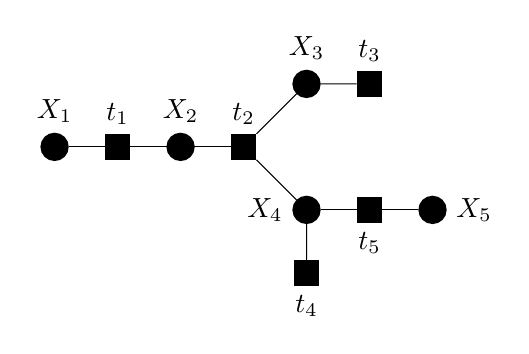
\begin{tikzpicture}[scale=0.8]
\tikzstyle{factor}=[rectangle,minimum size = 3mm, thick, draw =black,fill=black]
\tikzstyle{var}=[circle,minimum size = 3mm, thick, draw =black,fill=black]
\tikzstyle{second}=[circle, minimum size = 10mm, thick]
\tikzstyle{box}=[rectangle, draw=black!100]
\tikzstyle{connect}=[-latex, thick]
\draw[step=5cm];
	\node[var] (x_1) at (-1,0) [label=above:{$X_1$}]{};
	\node[factor] (t_1) at (0,0) [label=above:{$t_1$}]{};
	\node[var] (x_2) at (1,0) [label=above:{$X_2$}]{};
	\node[factor] (t_2) at (2,0) [label=above:{$t_2$}]{};
	\node[var] (x_3) at (3,1) [label=above:{$X_3$}]{};
	\node[factor] (t_3) at (4,1) [label=above:{$t_3$}]{};
	\node[var] (x_4) at (3,-1) [label=left:{$X_4$}]{};
	\node[factor] (t_4) at (3,-2) [label=below:{$t_4$}]{};
	\node[factor] (t_5) at (4,-1) [label=below:{$t_5$}]{};
	\node[var] (x_5) at (5,-1) [label=right:{$X_5$}]{};
	
	
	\path
		(x_1) edge []  (t_2) 
		(t_2) edge [] (x_3) 
		(x_3) edge [] (t_3)
		(t_2) edge [] (x_4)
		(t_4) edge [] (x_4)
		(x_4) edge [] (x_5);
		
\end{tikzpicture}
\end{figure}


}

\frame{
Since factors are non-negative, we may write:
\begin{align*}
\max_{\x\in\set{X}^5}\p{\X}(\x)&=\max_{\x\in\set{X}^5} t_1(x_1,x_2) t_2(x_2,x_3,x_4) t_3(x_3)t_4(x_4)t_5(x_4,x_5)\\\nonumber
&=\max_{(x_1,x_2,x_3,x_4)\in\set{X}^4}t_1(x_1,x_2) t_2(x_2,x_3,x_4) t_3(x_3)t_4(x_4)\color{darkblue}\underbrace{\max_{x_5\in\set{X}}t_5(x_4,x_5)}_{t_6(x_4)}\\\nonumber
&=\max_{(x_1,x_2)\in\set{X}^2}t_1(x_1,x_2) \color{darkred}\underbrace{\max_{(x_3,x_4)\in\set{X}^2} t_2(x_2,x_3,x_4) t_3(x_3)t_4(x_4)t_6(x_4)}_{t_7(x_2)}\\\nonumber
&=\max_{x_1\in\set{X}}\color{darkgreen}\underbrace{\max_{x_2\in\set{X}}t_1(x_1,x_2) t_7(x_2)}_{t_9(x_1)}=\color{black}\max_{x_1\in\set{X}}t_9(x_1),
\end{align*}

Computing the potentials $t_6(x_7), t_7(x_2)$ and $t_9(x_1)$ requires $\set{X}^2, \set{X}^3$ and $\set{X}^2$ operations.

}

\frame{
\frametitle{Backtracking}

We obtain $\x^*$ recursively
\begin{itemize}
\item $x_1^*=\displaystyle\arg\max_{x_1\in\set{X}}t_9(x_1)$.
\end{itemize}

\begin{itemize}
\item $x_2^*=\displaystyle\arg\max_{x_2\in\set{X}}t_1(x^*_1,x_2) t_7(x_2)$.
\end{itemize}

\begin{itemize}
\item $(x_3^*,x_4^*)=\displaystyle\arg\max_{x_3,x_4\in\set{X}^2}t_2(x^*_2,x_3,x_4) t_3(x_3)t_4(x_4)t_6(x_4)$.
\end{itemize}

\begin{itemize}
\item $x_5^*=\displaystyle\arg\max_{x_5\in\set{X}}t_5(x^*_4,x_5)$.
\end{itemize}

The cycle-free structure of the graph ensures that the maximal value (and its state) can be computed in time which scales linearly with the number of factors in the function.
}

\section{The Max-Product message passing algorithm}

\frame{
\frametitle{The Max-Product (MP) message passing algorithm}

\begin{itemize}
\item Message passing algorithm that defines a parallel procedure to avoid the sequential backtracking.
\item Consider
\begin{align*}
\p{\X}(\x)=\frac{1}{Z}\prod_{j\in\Iset{J}}t_j(\x_{j})\qquad x_i\in\set{X},~~ i=1,\ldots,n
\end{align*}
and assume that the FG associated is a tree. 
\end{itemize}


\begin{figure}
\centering
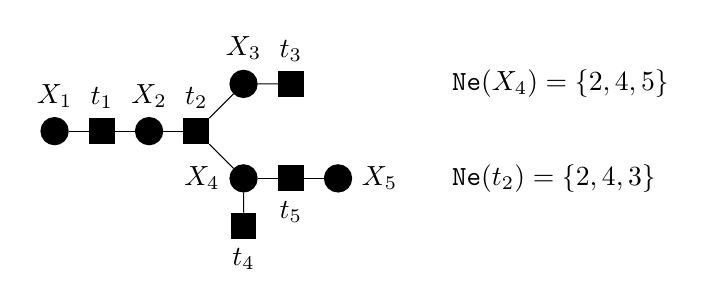
\begin{tikzpicture}[scale=0.6]
\tikzstyle{factor}=[rectangle,minimum size = 3mm, thick, draw =black,fill=black]
\tikzstyle{var}=[circle,minimum size = 3mm, thick, draw =black,fill=black]
\tikzstyle{second}=[circle, minimum size = 10mm, thick]
\tikzstyle{box}=[rectangle, draw=black!100]
\tikzstyle{connect}=[-latex, thick]
\draw[step=5cm];
	\node[var] (x_1) at (-1,0) [label=above:{$X_1$}]{};
	\node[factor] (t_1) at (0,0) [label=above:{$t_1$}]{};
	\node[var] (x_2) at (1,0) [label=above:{$X_2$}]{};
	\node[factor] (t_2) at (2,0) [label=above:{$t_2$}]{};
	\node[var] (x_3) at (3,1) [label=above:{$X_3$}]{};
	\node[factor] (t_3) at (4,1) [label=above:{$t_3$}]{};
	\node[var] (x_4) at (3,-1) [label=left:{$X_4$}]{};
	\node[factor] (t_4) at (3,-2) [label=below:{$t_4$}]{};
	\node[factor] (t_5) at (4,-1) [label=below:{$t_5$}]{};
	\node[var] (x_5) at (5,-1) [label=right:{$X_5$}]{};
	
     \node[] () at (7,1) [label=right:{$\Iset{Ne}(X_4)=\{2,4,5\}$}]{};
	\node[] () at (7,-1) [label=right:{$\Iset{Ne}(t_2)=\{2,4,3\}$}]{};

	\path
		(x_1) edge []  (t_2) 
		(t_2) edge [] (x_3) 
		(x_3) edge [] (t_3)
		(t_2) edge [] (x_4)
		(t_4) edge [] (x_4)
		(x_4) edge [] (x_5);
		
\end{tikzpicture}
\end{figure}


\begin{itemize}
\item $\Iset{Ne}(X_i)$ represents the index set of those factor nodes connected to the variable node $X_i$.
\item $\Iset{Ne}(t_j)$ the index set of those variable nodes connected to the factor node $t_j$
\end{itemize}

}


\frame{
\frametitle{Update rules}
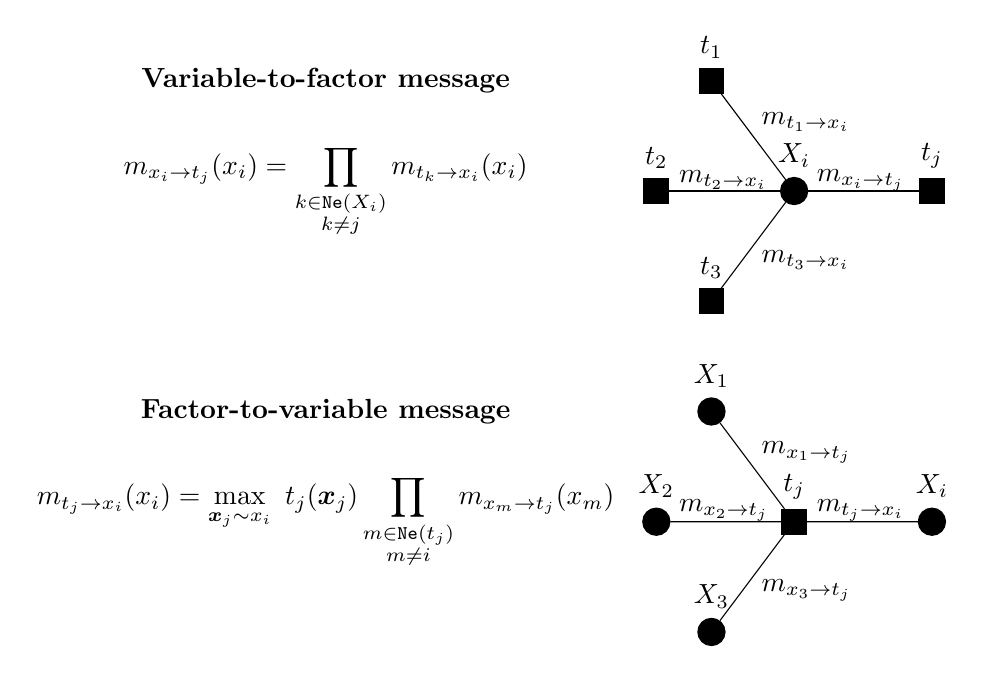
\begin{tikzpicture}[scale=0.7]
\tikzstyle{factor}=[rectangle,minimum size = 3mm, thick, draw =black, node distance = 16mm,fill=black]
\tikzstyle{var}=[circle,minimum size = 3mm, thick, draw =black, node distance = 16mm,fill=black]
\tikzstyle{second}=[circle, minimum size = 10mm, thick, node distance = 5mm]
\tikzstyle{box}=[rectangle, draw=black!100]
\tikzstyle{connect}=[-latex, thick]
\node[second] at (-6,2) [label=center:{\textbf{Variable-to-factor message}}]{};
\node[second] at (-6,0) [label=center:{$\displaystyle\mes{x_i}{t_j}(x_i)=\prod_{\substack{k\in\Iset{Ne}(X_i) \\ k\neq j}}\mes{t_k}{x_i}(x_i)$}]{};
%\node[second] at (-6,-2) [label=center:{\color{darkred}{$|\Iset{Ne}(X_i)|\times |\set{X}|$ pointwise multiplications}}]{};

\node[factor] (t_1) at (1,2) [label=above:$t_1$]{};
\node[factor] (t_2) at (0,0) [label=above:$t_2$]{};
\node[factor] (t_3) at (1,-2) [label=above:$t_3$]{};
\node[var] (x_i) at (2.5,0) [label=above:$X_i$]{};
\node[factor] (t_j) at (5,0) [label=above: $t_j$]{};
\node[second] (m1i) at (1,1.25) [label=right: $\mes{t_1}{x_i}$]{};
\node[second] (m2i) at (1,-1.25) [label=right: $\mes{t_3}{x_i}$]{};
\node[second] (m3i) at (-0.5,0.2) [label=right: $\mes{t_2}{x_i}$]{};
\node[second] (m4i) at (2,0.2) [label=right: $\mes{x_i}{t_j}$]{};

\path
	(t_1) edge (x_i)
	(t_2) edge (x_i)
	(t_3) edge (x_i)
	(x_i) edge (t_j);

\node[second] at (-6,-4) [label=center:{\textbf{Factor-to-variable message}}]{};
\node[second] at (-6,-6) [label=center:{$\displaystyle\mes{t_j}{x_i}(x_i)=\max_{\x_{j}\sim x_i}~ t_j(\x_{j})\prod_{\substack{m\in \Iset{Ne}(t_j) \\ m\neq i}}\mes{x_m}{t_j}(x_m)$}]{};
%\node[second] at (-6,-8) [label=center:{\color{darkred}{$|\Iset{Ne}(X_i)|\times |\set{X}|$ pointwise multiplications}}]{};
%\node[second] at (-6,-8) [label=center:{\color{darkred}{$|\Iset{Ne}(X_i)|^|\set{X}|$ additions}}]{};
\node[var] (t_12) at (1,-4) [label=above:$X_1$]{};
\node[var] (t_22) at (0,-6) [label=above:$X_2$]{};
\node[var] (t_32) at (1,-8) [label=above:$X_3$]{};
\node[factor] (x_i2) at (2.5,-6) [label=above:$t_j$]{};
\node[var] (t_j2) at (5,-6) [label=above: $X_i$]{};
\node[second] (m1i) at (1,-4.75) [label=right: $\mes{x_1}{t_j}$]{};
\node[second] (m2i) at (1,-7.25) [label=right: $\mes{x_3}{t_j}$]{};
\node[second] (m3i) at (-0.5,-5.8) [label=right: $\mes{x_2}{t_j}$]{};
\node[second] (m4i) at (2,-5.8) [label=right: $\mes{t_j}{x_i}$]{};

\path
	(t_12) edge (x_i2)
	(t_22) edge (x_i2)
	(t_32) edge (x_i2)
	(x_i2) edge (t_j2);
		
\end{tikzpicture}

}


\frame{
\frametitle{Update rules}
\begin{tikzpicture}[scale=0.7]
\tikzstyle{factor}=[rectangle,minimum size = 3mm, thick, draw =black, node distance = 16mm,fill=black]
\tikzstyle{var}=[circle,minimum size = 3mm, thick, draw =black, node distance = 16mm,fill=black]
\tikzstyle{second}=[circle, minimum size = 10mm, thick, node distance = 5mm]
\tikzstyle{box}=[rectangle, draw=black!100]
\tikzstyle{connect}=[-latex, thick]
\node[second] at (-6,2) [label=center:{\textbf{Variable-to-factor message}}]{};
\node[second] at (-6,0) [label=center:{$\displaystyle\mes{x_i}{t_j}(x_i)=\prod_{\substack{k\in\Iset{Ne}(X_i) \\ k\neq j}}\mes{t_k}{x_i}(x_i)$}]{};
\node[second] at (-6,-2) [label=center:{\color{darkred}{$|\Iset{Ne}(X_i)|\times |\set{X}|$ non-trivial multiplications}}]{};

\node[factor] (t_1) at (1,2) [label=above:$t_1$]{};
\node[factor] (t_2) at (0,0) [label=above:$t_2$]{};
\node[factor] (t_3) at (1,-2) [label=above:$t_3$]{};
\node[var] (x_i) at (2.5,0) [label=above:$X_i$]{};
\node[factor] (t_j) at (5,0) [label=above: $t_j$]{};
\node[second] (m1i) at (1,1.25) [label=right: $\mes{t_1}{x_i}$]{};
\node[second] (m2i) at (1,-1.25) [label=right: $\mes{t_3}{x_i}$]{};
\node[second] (m3i) at (-0.5,0.2) [label=right: $\mes{t_2}{x_i}$]{};
\node[second] (m4i) at (2,0.2) [label=right: $\mes{x_i}{t_j}$]{};

\path
	(t_1) edge (x_i)
	(t_2) edge (x_i)
	(t_3) edge (x_i)
	(x_i) edge (t_j);

\node[second] at (-6,-4) [label=center:{\textbf{Factor-to-variable message}}]{};
\node[second] at (-6,-6) [label=center:{$\displaystyle\mes{t_j}{x_i}(x_i)=\max_{\x_{j}\sim x_i}~ t_j(\x_{j})\prod_{\substack{m\in \Iset{Ne}(t_j) \\ m\neq i}}\mes{x_m}{t_j}(x_m)$}]{};
\node[second] at (-6,-8) [label=center:{\color{darkred}{$|\Iset{Ne}(t_j)|\times |\set{X}|$ non-trivial multiplications}}]{};
\node[second] at (-6,-9) [label=center:{\color{darkred}{$|\Iset{Ne}(t_j)|^{|\set{X}|}$ operations}}]{};
\node[var] (t_12) at (1,-4) [label=above:$X_1$]{};
\node[var] (t_22) at (0,-6) [label=above:$X_2$]{};
\node[var] (t_32) at (1,-8) [label=above:$X_3$]{};
\node[factor] (x_i2) at (2.5,-6) [label=above:$t_j$]{};
\node[var] (t_j2) at (5,-6) [label=above: $X_i$]{};
\node[second] (m1i) at (1,-4.75) [label=right: $\mes{x_1}{t_j}$]{};
\node[second] (m2i) at (1,-7.25) [label=right: $\mes{x_3}{t_j}$]{};
\node[second] (m3i) at (-0.5,-5.8) [label=right: $\mes{x_2}{t_j}$]{};
\node[second] (m4i) at (2,-5.8) [label=right: $\mes{t_j}{x_i}$]{};

\path
	(t_12) edge (x_i2)
	(t_22) edge (x_i2)
	(t_32) edge (x_i2)
	(x_i2) edge (t_j2);
		
\end{tikzpicture}

}



\frame{

Messages from leaf node factors are initialized to the factor and messages from the leaf variable nodes are set to all-one messages. 

\vspace{0.5cm}
As in the case of the SP update rules, any valid updating schedule has to verify the following:
\begin{enumerate}
\item After initialization, a message is sent for the first time from a node only when that node has received all requisite messages.
\item A message is updated and resent from a node to all its neighbours only when that node has received an updated incoming message. 
\end{enumerate}

\begin{exampleblock}{}
\noteB{Convergence is guaranteed for any tree factor graph.} After convergence,  the maximal state for each variable node is computed as follows:
\begin{align*}
x_i^*=\arg\max_{x\in\set{X}}\prod_{k\in\Iset{Ne}(X_i) }\mes{t_k}{x_i}(x_i)
\end{align*} 

\end{exampleblock}
}

\section{The Viterbi Algorithm}
\frame{
\frametitle{The Viterbi Algorithm}
Note that the MP algorithm applied to a \emph{state-space model} is equivalent to the Viterbi algorithm.

\begin{figure}
\vspace{0.5cm}
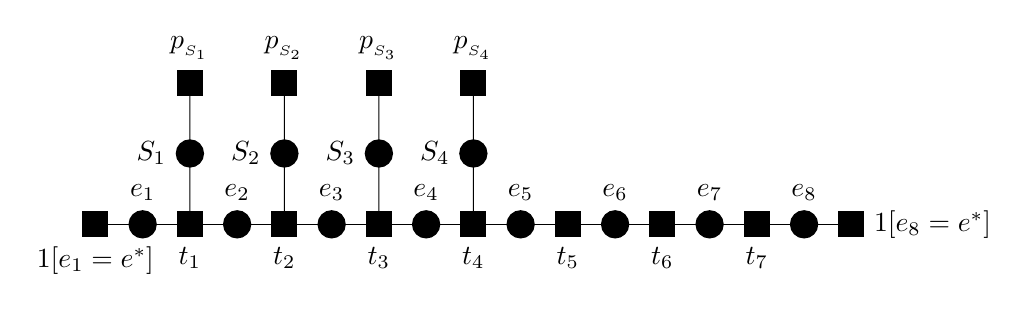
\begin{tikzpicture}[scale=0.3]
\tikzstyle{factor}=[rectangle,minimum size = 3mm, thick, draw =black,fill=black]
\tikzstyle{var}=[circle,minimum size = 3mm, thick, draw =black,fill=black]
\tikzstyle{connect}=[-latex, thick]

	
	\node[factor] (tphi0) at (0,0) [label=below:{$\ind[\st{1}=\st{}^*]$}]{};
	\node[var] (phi0) at (2,0) [label=above:{$\st{1}$}]{};
	\node[factor] (tphi1) at (4,0) [label=below:{$t_1$}]{};
	\node[var] (s0) at (4,3) [label=left:{$S_1$}]{};
	\node[factor] (fs0) at (4,6) [label=above:{$\p{S_1}$}]{};
	
	\node[var] (phi1) at (6,0) [label=above:{$\st{2}$}]{};
	\node[factor] (tphi2) at (8,0) [label=below:{$t_2$}]{};
	\node[var] (s1) at (8,3) [label=left:{$S_2$}]{};
	\node[factor] (fs1) at (8,6) [label=above:{$\p{S_2}$}]{};	

	
	\node[var] (phi2) at (10,0) [label=above:{$\st{3}$}]{};
	\node[factor] (tphi3) at (12,0) [label=below:{$t_3$}]{};
		\node[var] (s2) at (12,3) [label=left:{$S_3$}]{};
	\node[factor] (fs2) at (12,6) [label=above:{$\p{S_3}$}]{};		
	
	\node[var] (phi3) at (14,0) [label=above:{$\st{4}$}]{};
	\node[factor] (tphi4) at (16,0) [label=below:{$t_4$}]{};
	\node[var] (s3) at (16,3) [label=left:{$S_4$}]{};	
	\node[factor] (fs3) at (16,6) [label=above:{$\p{S_4}$}]{};
	
	\node[var] (phi4) at (18,0) [label=above:{$\st{5}$}]{};
	\node[factor] (tphi5) at (20,0) [label=below:{$t_5$}]{};
	%\node[var] (s4) at (20,3) [label=left:{$S_5$}]{};	
	%\node[factor] (fs4) at (20,6) [label=above:{$\p{S_5}$}]{};	
	
	%\node[factor] (fs5) at (24,6) [label=above:{$\p{S_6}$}]{};	
	%\node[var] (s5) at (24,3) [label=left:{$S_6$}]{};	
	\node[var] (phi5) at (22,0) [label=above:{$\st{6}$}]{};
	\node[factor] (tphi6) at (24,0) [label=below:{$t_6$}]{};	
	
	%\node[factor] (fs6) at (28,6) [label=above:{$\p{S_7}$}]{};	
	%\node[var] (s6) at (28,3) [label=left:{$S_7$}]{};	
	\node[var] (phi6) at (26,0) [label=above:{$\st{7}$}]{};
	\node[factor] (tphi7) at (28,0) [label=below:{$t_7$}]{};
	\node[var] (phi7) at (30,0) [label=above:{$\st{8}$}]{};
	\node[factor] (tphi8) at (32,0) [label=right:{$\ind[\st{8}=\st{}^*]$}]{};
	
	\path
		(tphi0) edge [] (tphi8)
		(fs0) edge [] (tphi1)
		(fs1) edge [] (tphi2)
		(fs2) edge [] (tphi3)
		(fs3) edge [] (tphi4);	
				
		
	
\end{tikzpicture}
\caption{Factor graph associated tothe joint distribution of symbols and states in the scenario of tramission of QAM symbols over an ISI channel. $\chl=3$ and $\t=4$.}
\end{figure}
}


\end{document}

